%(BEGIN_QUESTION)
% Copyright 2007, Tony R. Kuphaldt, released under the Creative Commons Attribution License (v 1.0)
% This means you may do almost anything with this work of mine, so long as you give me proper credit

Tegn kvalitativt de individuelle responsene for proporsjonal-, integral- og derivatledd i en PID-regulator for følgende inngangsbetingelser, forutsatt {\it direkte} reguleringsretning. Bruk heltrukket linje for proporsjonal, stiplet linje for integral og prikket linje for derivat:

$$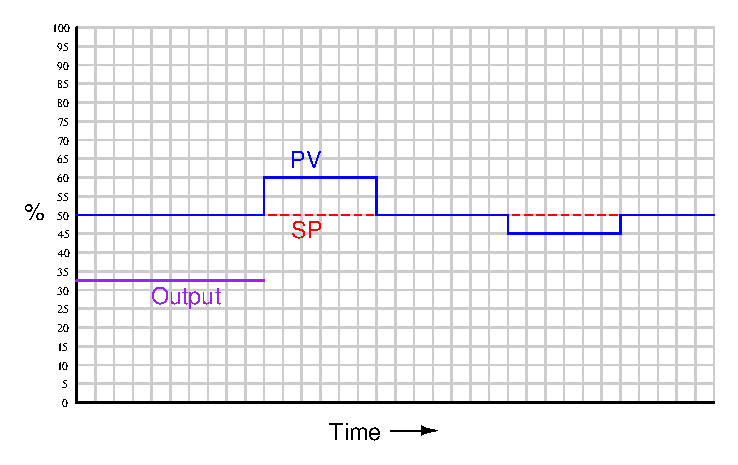
\includegraphics[width=15.5cm]{i01637x01.eps}$$

Tegn deretter en sluttgraf for regulatorens utgang, som viser hvordan P-, I- og D-leddene kombineres til en sammensatt kurveform:

$$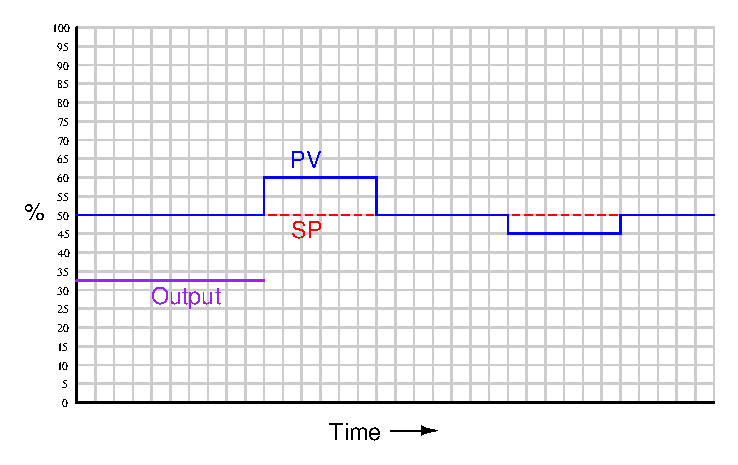
\includegraphics[width=15.5cm]{i01637x01.eps}$$

\vskip 20pt \vbox{\hrule \hbox{\strut \vrule{} {\bf Forslag til sokratisk diskusjon} \vrule} \hrule}

\begin{itemize}
\item{} Mange studenter opplever at det er mye vanskeligere å summere alle tre reguleringsvirkningene enn å plotte hver av de tre responsene separat. Lag en problemløsningsstrategi som sikrer at summeringen alltid blir riktig!
\end{itemize}

\underbar{file i01637}
%(END_QUESTION)





%(BEGIN_ANSWER)

Grafen for regulatorutgangen som vises her er kun {\it kvalitativ}. Selv om den er tegnet i skala (dvs. alle endringer i utgangen er korrekt skalert relativt til hverandre), er selve skalaen vilkårlig og trenger derfor ikke å samsvare med skalaen i din skisse:

\vskip 10pt

Individuelle P-, I- og D-responser plottet:

$$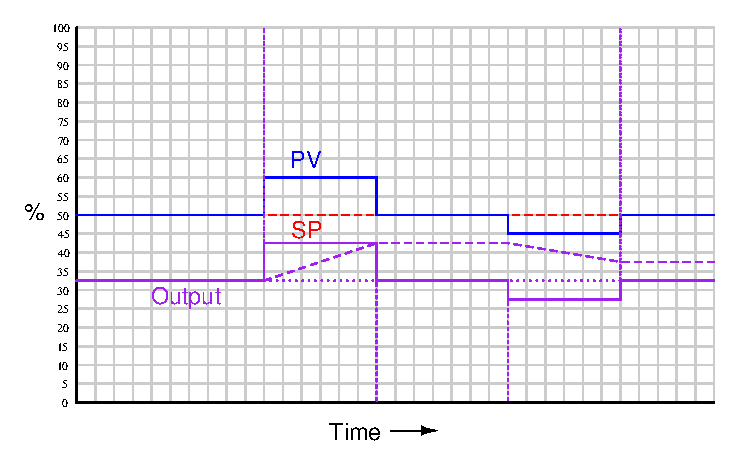
\includegraphics[width=15.5cm]{i01637x02.eps}$$

Sluttgraf for utgangssignal:

$$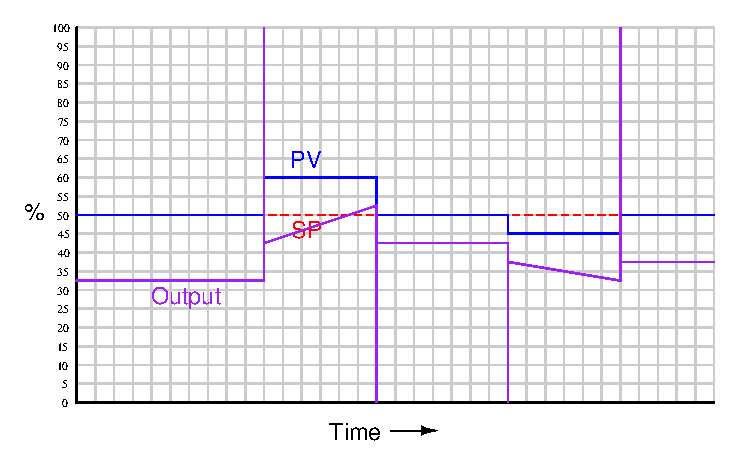
\includegraphics[width=15.5cm]{i01637x03.eps}$$

%(END_ANSWER)





%(BEGIN_NOTES)



%INDEX% Control, proportional + integral + derivative: graphing controller response

%(END_NOTES)
